\problem{}

You are a commander about to participate in an simulated combat exercise.  
You have $n$ elite soldiers under your command, numbered from $1$ to $n$.

There are two main battle zones on the exercise map: Zone A and Zone B.  
The battlefield conditions differ between these two zones, so the same soldier may have different combat effectiveness depending on where they are deployed:
\begin{itemize}
    \item If the $i$-th soldier is deployed to Zone A, he contributes $a_i$ combat power.
    \item If deployed to Zone B, he contributes $b_i$ combat power.
\end{itemize}

Each soldier can only be assigned to one battle zone.

There are $m$ synergistic groups, denoted as $g_1, g_2, \dots, g_m$, where each group contains several specific soldiers.  
If all members of group $g_i$ are deployed to the same zone, the following synergy bonuses apply:
\begin{itemize}
    \item If all are deployed to Zone A, an additional $c_{i,1}$ combat power is gained.
    \item If all are deployed to Zone B, an additional $c_{i,2}$ combat power is gained.
\end{itemize}

Your task is to deploy all soldiers to Zones A and B in such a way that the total combat power (the sum of the contributions of all soldiers plus the synergy bonuses) is maximized.

For example,
\[
n = 3, \quad a = [4, 2, 1], \quad b = [2, 3, 3],
\]
\[
m = 1, \quad g_1 = \{1, 2\}, \quad c_1 = [4, 2].
\]
If soldiers 1 and 2 are deployed to Zone A and soldier 3 is deployed to Zone B,  
the maximum total combat power is
\[
4 + 2 + 4 + 3 = 13.
\]

Please use \textbf{network flow} to solve this problem.  
\textbf{Your answer should include the following:}
\begin{enumerate}
    \item The construction of the nodes in the graph.
    \item The way edges are connected and how capacities are defined.
    \item How to calculate the maximum total combat power.
    \item A diagram showing the graph constructed for the example data (similar to the illustration in \emph{Lecture 9, page 16}).
\end{enumerate}

\newpage
\noindent \textbf{Solution}:

\noindent \textbf{1 The construction of the nodes in the graph.}


\begin{itemize}
    \item Source \( s \) represents Zone A.
    \item Sink \( t \) represents Zone B.
    \item For each soldier \( i= 1\dots n \), a node \( u_i \).
    \item For each group \( g_k = 1\dots m \), two auxiliary nodes:
        \begin{itemize}
            \item \( p_k \): ``all in A'' event node.
            \item \( q_k \): ``all in B'' event node.
        \end{itemize}
\end{itemize}

\noindent \textbf{2 The way edges are connected and how capacities are defined.}

\noindent Soldier choice edges

\begin{itemize}
    \item \( s \to u_i \), capacity \( a_i \): cut if soldier \( i \) not in A (lose \( a_i \)).
    \item \( u_i \to t \), capacity \( b_i \): cut if soldier \( i \) not in B (lose \( b_i \)).
\end{itemize}

\noindent Synergy bonus edges


\begin{itemize}
    \item \( s \to p_k \), capacity \( c_{k,1} \): cut if not all in A (lose \( c_{k,1} \)).
    \item \( q_k \to t \), capacity \( c_{k,2} \): cut if not all in B (lose \( c_{k,2} \)).
\end{itemize}

\noindent Enforcement edges (infinite capacity)

\begin{itemize}
    \item \( p_k \to u_i \) for all \( i \in g_k \), capacity \( \infty \): ensures \( p_k \) in \( s \)-side only if all \( u_i \) in \( s \)-side.
    \item \( u_i \to q_k \) for all \( i \in g_k \), capacity \( \infty \): ensures \( q_k \) in \( t \)-side only if all \( u_i \) in \( t \)-side.
\end{itemize}


\noindent \textbf{3 How to calculate the maximum total combat power}

The core idea of this problem is to transform the maximization of combat power 
into a minimization of lost potential via a minimum cut model. 
We first calculate the theoretical maximum sum if all individual contributions and all synergy 
 bonuses could be obtained simultaneously. 
 Since deployment constraints make this impossible, we build a flow network where the capacities of the edges 
 represent the penalties for not achieving certain contributions. 
 The minimum cut of this network corresponds to the minimum total loss 
 we must incur. Therefore, subtracting this min-cut value 
 from the theoretical maximum 
 yields the actual maximum achievable combat power.

We use the \textbf{min-cut} model in a flow network:

\begin{enumerate}
    \item \textbf{Construct the graph} as described, with:
    \begin{itemize}
        \item Source \( s \) and sink \( t \)
        \item Soldier nodes \( u_i \)
        \item Group event nodes \( p_k \) (all-in-A) and \( q_k \) (all-in-B)
        \item Edges with capacities \( a_i, b_i, c_{k,1}, c_{k,2}, \infty \) as defined
    \end{itemize}
    
    \item \textbf{Compute the maximum flow} from \( s \) to \( t \) (using any max-flow algorithm, e.g., Edmonds–Karp or Dinic)
    
    \item \textbf{Define the total ``potential'' sum}:
    \[
    \text{Sum} = \sum_{i=1}^n (a_i + b_i) + \sum_{k=1}^m (c_{k,1} + c_{k,2})
    \]
    This is the total combat power if we could get all individual contributions and all synergy bonuses simultaneously (which is impossible due to deployment constraints)
    
    \item \textbf{Then:}
    \[
    \text{Max Combat Power} = \text{Sum} - \text{Max Flow Value}
    \]
    Here, the \textbf{max flow value} equals the \textbf{min-cut capacity}, which represents the minimum total ``loss'' of combat power we must suffer due to conflicting deployment choices
\end{enumerate}

\noindent \textbf{4 A diagram showing the graph constructed for the example data}

\begin{figure}[h]
    \centering
    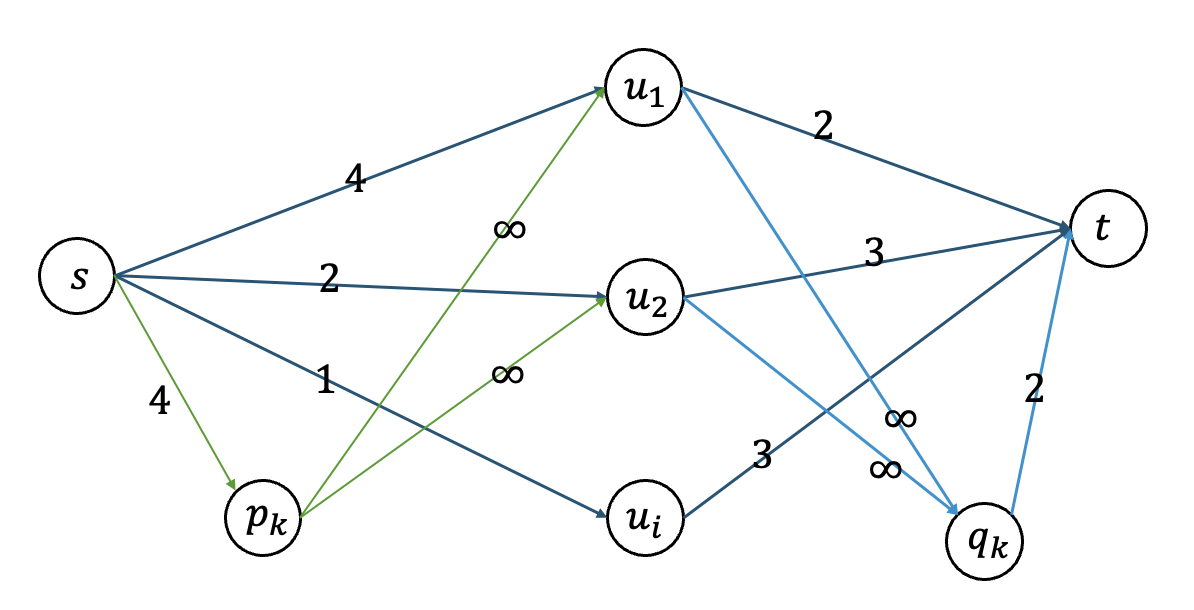
\includegraphics[width=\linewidth]{figure/1761915145315.png}

\end{figure}
$\text{Max Combat Power}= \sum_{i=1}^n (a_i + b_i) + \sum_{k=1}^m (c_{k,1} + c_{k,2})- \text{Max Flow Value}\\=(4+2+1+2+3+3)+(2+4)-8=13$
\newpage